
%% bare_conf.tex
%% V1.3
%% 2007/01/11
%% by Michael Shell
%% See:
%% http://www.michaelshell.org/
%% for current contact information.
%%
%% This is a skeleton file demonstrating the use of IEEEtran.cls
%% (requires IEEEtran.cls version 1.7 or later) with an IEEE conference paper.
%%
%% Support sites:
%% http://www.michaelshell.org/tex/ieeetran/
%% http://www.ctan.org/tex-archive/macros/latex/contrib/IEEEtran/
%% and
%% http://www.ieee.org/

%%*************************************************************************
%% Legal Notice:
%% This code is offered as-is without any warranty either expressed or
%% implied; without even the implied warranty of MERCHANTABILITY or
%% FITNESS FOR A PARTICULAR PURPOSE! 
%% User assumes all risk.
%% In no event shall IEEE or any contributor to this code be liable for
%% any damages or losses, including, but not limited to, incidental,
%% consequential, or any other damages, resulting from the use or misuse
%% of any information contained here.
%%
%% All comments are the opinions of their respective authors and are not
%% necessarily endorsed by the IEEE.
%%
%% This work is distributed under the LaTeX Project Public License (LPPL)
%% ( http://www.latex-project.org/ ) version 1.3, and may be freely used,
%% distributed and modified. A copy of the LPPL, version 1.3, is included
%% in the base LaTeX documentation of all distributions of LaTeX released
%% 2003/12/01 or later.
%% Retain all contribution notices and credits.
%% ** Modified files should be clearly indicated as such, including  **
%% ** renaming them and changing author support contact information. **
%%
%% File list of work: IEEEtran.cls, IEEEtran_HOWTO.pdf, bare_adv.tex,
%%                    bare_conf.tex, bare_jrnl.tex, bare_jrnl_compsoc.tex
%%*************************************************************************

% *** Authors should verify (and, if needed, correct) their LaTeX system  ***
% *** with the testflow diagnostic prior to trusting their LaTeX platform ***
% *** with production work. IEEE's font choices can trigger bugs that do  ***
% *** not appear when using other class files.                            ***
% The testflow support page is at:
% http://www.michaelshell.org/tex/testflow/



% Note that the a4paper option is mainly intended so that authors in
% countries using A4 can easily print to A4 and see how their papers will
% look in print - the typesetting of the document will not typically be
% affected with changes in paper size (but the bottom and side margins will).
% Use the testflow package mentioned above to verify correct handling of
% both paper sizes by the user's LaTeX system.
%
% Also note that the "draftcls" or "draftclsnofoot", not "draft", option
% should be used if it is desired that the figures are to be displayed in
% draft mode.
%
\documentclass[conference]{IEEEtran}
% Add the compsoc option for Computer Society conferences.
%
% If IEEEtran.cls has not been installed into the LaTeX system files,
% manually specify the path to it like:
% \documentclass[conference]{../sty/IEEEtran}





% Some very useful LaTeX packages include:
% (uncomment the ones you want to load)


% *** MISC UTILITY PACKAGES ***
%
%\usepackage{ifpdf}
% Heiko Oberdiek's ifpdf.sty is very useful if you need conditional
% compilation based on whether the output is pdf or dvi.
% usage:
% \ifpdf
%   % pdf code
% \else
%   % dvi code
% \fi
% The latest version of ifpdf.sty can be obtained from:
% http://www.ctan.org/tex-archive/macros/latex/contrib/oberdiek/
% Also, note that IEEEtran.cls V1.7 and later provides a builtin
% \ifCLASSINFOpdf conditional that works the same way.
% When switching from latex to pdflatex and vice-versa, the compiler may
% have to be run twice to clear warning/error messages.






% *** CITATION PACKAGES ***
%
%\usepackage{cite}
% cite.sty was written by Donald Arseneau
% V1.6 and later of IEEEtran pre-defines the format of the cite.sty package
% \cite{} output to follow that of IEEE. Loading the cite package will
% result in citation numbers being automatically sorted and properly
% "compressed/ranged". e.g., [1], [9], [2], [7], [5], [6] without using
% cite.sty will become [1], [2], [5]--[7], [9] using cite.sty. cite.sty's
% \cite will automatically add leading space, if needed. Use cite.sty's
% noadjust option (cite.sty V3.8 and later) if you want to turn this off.
% cite.sty is already installed on most LaTeX systems. Be sure and use
% version 4.0 (2003-05-27) and later if using hyperref.sty. cite.sty does
% not currently provide for hyperlinked citations.
% The latest version can be obtained at:
% http://www.ctan.org/tex-archive/macros/latex/contrib/cite/
% The documentation is contained in the cite.sty file itself.


\usepackage{enumerate}
\usepackage{rotating}
\usepackage{url}

% *** GRAPHICS RELATED PACKAGES ***
%
\ifCLASSINFOpdf
  % \usepackage[pdftex]{graphicx}
  % declare the path(s) where your graphic files are
  % \graphicspath{{../pdf/}{../jpeg/}}
  % and their extensions so you won't have to specify these with
  % every instance of \includegraphics
  % \DeclareGraphicsExtensions{.pdf,.jpeg,.png}
\else
  % or other class option (dvipsone, dvipdf, if not using dvips). graphicx
  % will default to the driver specified in the system graphics.cfg if no
  % driver is specified.
  % \usepackage[dvips]{graphicx}
  % declare the path(s) where your graphic files are
  % \graphicspath{{../eps/}}
  % and their extensions so you won't have to specify these with
  % every instance of \includegraphics
  % \DeclareGraphicsExtensions{.eps}
\fi
% graphicx was written by David Carlisle and Sebastian Rahtz. It is
% required if you want graphics, photos, etc. graphicx.sty is already
% installed on most LaTeX systems. The latest version and documentation can
% be obtained at: 
% http://www.ctan.org/tex-archive/macros/latex/required/graphics/
% Another good source of documentation is "Using Imported Graphics in
% LaTeX2e" by Keith Reckdahl which can be found as epslatex.ps or
% epslatex.pdf at: http://www.ctan.org/tex-archive/info/
%
% latex, and pdflatex in dvi mode, support graphics in encapsulated
% postscript (.eps) format. pdflatex in pdf mode supports graphics
% in .pdf, .jpeg, .png and .mps (metapost) formats. Users should ensure
% that all non-photo figures use a vector format (.eps, .pdf, .mps) and
% not a bitmapped formats (.jpeg, .png). IEEE frowns on bitmapped formats
% which can result in "jaggedy"/blurry rendering of lines and letters as
% well as large increases in file sizes.
%
% You can find documentation about the pdfTeX application at:
% http://www.tug.org/applications/pdftex





% *** MATH PACKAGES ***
%
%\usepackage[cmex10]{amsmath}
% A popular package from the American Mathematical Society that provides
% many useful and powerful commands for dealing with mathematics. If using
% it, be sure to load this package with the cmex10 option to ensure that
% only type 1 fonts will utilized at all point sizes. Without this option,
% it is possible that some math symbols, particularly those within
% footnotes, will be rendered in bitmap form which will result in a
% document that can not be IEEE Xplore compliant!
%
% Also, note that the amsmath package sets \interdisplaylinepenalty to 10000
% thus preventing page breaks from occurring within multiline equations. Use:
%\interdisplaylinepenalty=2500
% after loading amsmath to restore such page breaks as IEEEtran.cls normally
% does. amsmath.sty is already installed on most LaTeX systems. The latest
% version and documentation can be obtained at:
% http://www.ctan.org/tex-archive/macros/latex/required/amslatex/math/





% *** SPECIALIZED LIST PACKAGES ***
%
%\usepackage{algorithmic}
% algorithmic.sty was written by Peter Williams and Rogerio Brito.
% This package provides an algorithmic environment fo describing algorithms.
% You can use the algorithmic environment in-text or within a figure
% environment to provide for a floating algorithm. Do NOT use the algorithm
% floating environment provided by algorithm.sty (by the same authors) or
% algorithm2e.sty (by Christophe Fiorio) as IEEE does not use dedicated
% algorithm float types and packages that provide these will not provide
% correct IEEE style captions. The latest version and documentation of
% algorithmic.sty can be obtained at:
% http://www.ctan.org/tex-archive/macros/latex/contrib/algorithms/
% There is also a support site at:
% http://algorithms.berlios.de/index.html
% Also of interest may be the (relatively newer and more customizable)
% algorithmicx.sty package by Szasz Janos:
% http://www.ctan.org/tex-archive/macros/latex/contrib/algorithmicx/




% *** ALIGNMENT PACKAGES ***
%
%\usepackage{array}
% Frank Mittelbach's and David Carlisle's array.sty patches and improves
% the standard LaTeX2e array and tabular environments to provide better
% appearance and additional user controls. As the default LaTeX2e table
% generation code is lacking to the point of almost being broken with
% respect to the quality of the end results, all users are strongly
% advised to use an enhanced (at the very least that provided by array.sty)
% set of table tools. array.sty is already installed on most systems. The
% latest version and documentation can be obtained at:
% http://www.ctan.org/tex-archive/macros/latex/required/tools/


%\usepackage{mdwmath}
%\usepackage{mdwtab}
% Also highly recommended is Mark Wooding's extremely powerful MDW tools,
% especially mdwmath.sty and mdwtab.sty which are used to format equations
% and tables, respectively. The MDWtools set is already installed on most
% LaTeX systems. The lastest version and documentation is available at:
% http://www.ctan.org/tex-archive/macros/latex/contrib/mdwtools/


% IEEEtran contains the IEEEeqnarray family of commands that can be used to
% generate multiline equations as well as matrices, tables, etc., of high
% quality.


%\usepackage{eqparbox}
% Also of notable interest is Scott Pakin's eqparbox package for creating
% (automatically sized) equal width boxes - aka "natural width parboxes".
% Available at:
% http://www.ctan.org/tex-archive/macros/latex/contrib/eqparbox/





% *** SUBFIGURE PACKAGES ***
%\usepackage[tight,footnotesize]{subfigure}
% subfigure.sty was written by Steven Douglas Cochran. This package makes it
% easy to put subfigures in your figures. e.g., "Figure 1a and 1b". For IEEE
% work, it is a good idea to load it with the tight package option to reduce
% the amount of white space around the subfigures. subfigure.sty is already
% installed on most LaTeX systems. The latest version and documentation can
% be obtained at:
% http://www.ctan.org/tex-archive/obsolete/macros/latex/contrib/subfigure/
% subfigure.sty has been superceeded by subfig.sty.



%\usepackage[caption=false]{caption}
%\usepackage[font=footnotesize]{subfig}
% subfig.sty, also written by Steven Douglas Cochran, is the modern
% replacement for subfigure.sty. However, subfig.sty requires and
% automatically loads Axel Sommerfeldt's caption.sty which will override
% IEEEtran.cls handling of captions and this will result in nonIEEE style
% figure/table captions. To prevent this problem, be sure and preload
% caption.sty with its "caption=false" package option. This is will preserve
% IEEEtran.cls handing of captions. Version 1.3 (2005/06/28) and later 
% (recommended due to many improvements over 1.2) of subfig.sty supports
% the caption=false option directly:
%\usepackage[caption=false,font=footnotesize]{subfig}
%
% The latest version and documentation can be obtained at:
% http://www.ctan.org/tex-archive/macros/latex/contrib/subfig/
% The latest version and documentation of caption.sty can be obtained at:
% http://www.ctan.org/tex-archive/macros/latex/contrib/caption/




% *** FLOAT PACKAGES ***
%
%\usepackage{fixltx2e}
% fixltx2e, the successor to the earlier fix2col.sty, was written by
% Frank Mittelbach and David Carlisle. This package corrects a few problems
% in the LaTeX2e kernel, the most notable of which is that in current
% LaTeX2e releases, the ordering of single and double column floats is not
% guaranteed to be preserved. Thus, an unpatched LaTeX2e can allow a
% single column figure to be placed prior to an earlier double column
% figure. The latest version and documentation can be found at:
% http://www.ctan.org/tex-archive/macros/latex/base/



%\usepackage{stfloats}
% stfloats.sty was written by Sigitas Tolusis. This package gives LaTeX2e
% the ability to do double column floats at the bottom of the page as well
% as the top. (e.g., "\begin{figure*}[!b]" is not normally possible in
% LaTeX2e). It also provides a command:
%\fnbelowfloat
% to enable the placement of footnotes below bottom floats (the standard
% LaTeX2e kernel puts them above bottom floats). This is an invasive package
% which rewrites many portions of the LaTeX2e float routines. It may not work
% with other packages that modify the LaTeX2e float routines. The latest
% version and documentation can be obtained at:
% http://www.ctan.org/tex-archive/macros/latex/contrib/sttools/
% Documentation is contained in the stfloats.sty comments as well as in the
% presfull.pdf file. Do not use the stfloats baselinefloat ability as IEEE
% does not allow \baselineskip to stretch. Authors submitting work to the
% IEEE should note that IEEE rarely uses double column equations and
% that authors should try to avoid such use. Do not be tempted to use the
% cuted.sty or midfloat.sty packages (also by Sigitas Tolusis) as IEEE does
% not format its papers in such ways.





% *** PDF, URL AND HYPERLINK PACKAGES ***
%
%\usepackage{url}
% url.sty was written by Donald Arseneau. It provides better support for
% handling and breaking URLs. url.sty is already installed on most LaTeX
% systems. The latest version can be obtained at:
% http://www.ctan.org/tex-archive/macros/latex/contrib/misc/
% Read the url.sty source comments for usage information. Basically,
% \url{my_url_here}.





% *** Do not adjust lengths that control margins, column widths, etc. ***
% *** Do not use packages that alter fonts (such as pslatex).         ***
% There should be no need to do such things with IEEEtran.cls V1.6 and later.
% (Unless specifically asked to do so by the journal or conference you plan
% to submit to, of course. )


% correct bad hyphenation here
\hyphenation{op-tical net-works semi-conduc-tor}


\begin{document}
%
% paper title
% can use linebreaks \\ within to get better formatting as desired
\title{Active Code Completion}


% author names and affiliations
% use a multiple column layout for up to three different
% affiliations
\author{\IEEEauthorblockN{Cyrus Omar, YoungSeok Yoon, Thomas D. LaToza, Brad A. Myers}
\IEEEauthorblockA{School of Computer Science\\
Carnegie Mellon University\\
Pittsburgh, PA, USA\\
\{comar,youngseok,tlatoza,bam\}@cs.cmu.edu}
\texttt{\url{https://github.com/cyrus~/graphite}}
}

% conference papers do not typically use \thanks and this command
% is locked out in conference mode. If really needed, such as for
% the acknowledgment of grants, issue a \IEEEoverridecommandlockouts
% after \documentclass

% for over three affiliations, or if they all won't fit within the width
% of the page, use this alternative format:
% 
%\author{\IEEEauthorblockN{Michael Shell\IEEEauthorrefmark{1},
%Homer Simpson\IEEEauthorrefmark{2},
%James Kirk\IEEEauthorrefmark{3}, 
%Montgomery Scott\IEEEauthorrefmark{3} and
%Eldon Tyrell\IEEEauthorrefmark{4}}
%\IEEEauthorblockA{\IEEEauthorrefmark{1}School of Electrical and Computer Engineering\\
%Georgia Institute of Technology,
%Atlanta, Georgia 30332--0250\\ Email: see http://www.michaelshell.org/contact.html}
%\IEEEauthorblockA{\IEEEauthorrefmark{2}Twentieth Century Fox, Springfield, USA\\
%Email: homer@thesimpsons.com}
%\IEEEauthorblockA{\IEEEauthorrefmark{3}Starfleet Academy, San Francisco, California 96678-2391\\
%Telephone: (800) 555--1212, Fax: (888) 555--1212}
%\IEEEauthorblockA{\IEEEauthorrefmark{4}Tyrell Inc., 123 Replicant Street, Los Angeles, California 90210--4321}}




% use for special paper notices
%\IEEEspecialpapernotice{(Invited Paper)}




% make the title area
\maketitle


% IEEEtran.cls defaults to using nonbold math in the Abstract.
% This preserves the distinction between vectors and scalars. However,
% if the conference you are submitting to favors bold math in the abstract,
% then you can use LaTeX's standard command \boldmath at the very start
% of the abstract to achieve this. Many IEEE journals/conferences frown on
% math in the abstract anyway.

% no keywords




% For peer review papers, you can put extra information on the cover
% page as needed:
% \ifCLASSOPTIONpeerreview
% \begin{center} \bfseries EDICS Category: 3-BBND \end{center}
% \fi
%
% For peerreview papers, this IEEEtran command inserts a page break and
% creates the second title. It will be ignored for other modes.
\IEEEpeerreviewmaketitle



\section{Introduction}


Software developers today make heavy use of the code completion features available in modern code editors \cite{murphy_how_2006}. By navigating and selecting from a floating menu containing the names of variables, fields, methods, types and code snippets, a developer can avoid many common spelling and logic errors, avoid unnecessary keystrokes and explore unfamiliar APIs without leaving the editor window. To ensure that the items featured in this menu are relevant, the editor conducts a static analysis of the surrounding code context. %In many editors, an area adjacent to this menu displays documentation associated with the  currently highlighted item.

Several refinements and additions to the code completion menu have been previously suggested in the literature. These have focused on using additional sources of information, such as databases of usage history \cite{robbes_how_2008}, examples extracted from code repositories \cite{bruch_learning_2009} and crowdsourced information \cite{mooty_calcite:_2010}, to increase the relevance and sophistication of the featured items. Empirical evidence presented in these studies suggests that these enhancements further improve developer productivity.

In this paper, we propose a complementary technique called {\it active code completion}. When the developer invokes the code completion menu, the editor looks for a {\it palette definition} associated with the type of the expression being entered. If found, an option to use this palette is added to the code completion menu.
When the developer selects this option, source code is not inserted immediately. Instead, the palette definition takes control of the code completion interface. The developer can then interact with this interface to provide parameters and other information related to her intent, and receive immediate feedback about the effect these choices will have on the object's behavior. When the developer indicates that she is satisfied with these choices, the palette generates code that is inserted at the cursor. 

Before designing and implementing such a system, we sought to address the following questions:

\begin{itemize}
\item What are some specific use cases for active code completion in a professional development setting? 
\item Which functional criteria are common to types that would benefit from an associated palette?
\item What usability criteria should inform palette interface designs in this context?
\item Which capabilities must the active code completion architecture have to enable these use cases and designs?
\end{itemize}

To answer these questions, we began by conducting a large online survey of professional developers. Their responses revealed a number of interesting use cases and non-trivial design constraints for active code completion systems. 

Based on this information, we designed and implemented an Eclipse plug-in that provides active code completion for the Java language, and implemented some example palettes atop this system. 
Finally, we evaluated the usefulness of one such palette, designed to assist developers as they write regular expressions, with a controlled lab study. The data and observations from this study provide empirical evidence in support of the view that an active code completion system would be useful to professional developers.

\section{Developer Survey}
The subject pool for the preliminary survey consisted primarily of visitors to a large programming-oriented 
collaborative filtering forum\footnote{http://www.reddit.com/r/programming}.
A small number of participants were also recruited using a
mass email to local computer science graduate students. Participants were asked to take an online survey taking  approximately 20 minutes to complete and background information collected from the 475 participants indicated that the overwhelming majority of participants were professional developers.

Participants were shown three mockup palettes, along with mockups of the invocation procedure described above, for classes representing colors, regular expressions and SQL queries. They were asked to indicate whether they would find these palettes useful. Their responses are summarized in Figure 1 and indicate that these developers found the concept potentially useful, with a particular preference for the palette shown for regular expressions.

Participants were also asked to provide free-form comments on each palette. These responses revealed a number of concerns about this system. These include issues related to handling separation of concerns, reinvocation, palette settings and state, interactions between the palette and the code context, language and editor independence, and keyboard navigability. These concerns strongly influenced the design of the code completion system described in the next section.

Finally, we solicited suggestions for classes that may benefit from an associated palette. We received a number of interesting suggestions, which we broadly classified into categories. Examples include classes that would benefit from an alternative syntax (e.g. dictionaries), where the implications of a parameter choice are difficult to predict (e.g. 3D transformation matrices), where the instantiation procedure is non-trivial (e.g. factory methods) and where parameters could be provided by example (e.g. key combinations).
\begin{figure*}\begin{center}
  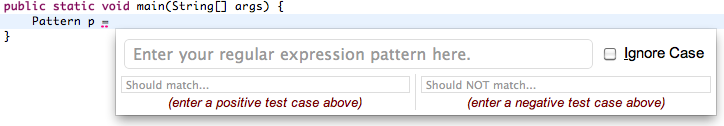
\includegraphics[scale=.4]{regex.png}\end{center}
  %\caption{Test}
  \vspace{-15pt}
  \end{figure*}

\begin{figure}
\begin{tabular}{crccccc}\\\\
\textsc{class}
& 
& \begin{rotate}{20}Nearly every time\end{rotate}
& \begin{rotate}{20}Most of the time\end{rotate}
& \begin{rotate}{20}Some of the time\end{rotate}
& \begin{rotate}{20}Rarely\end{rotate}
& \begin{turn}{20}Never\end{turn}\\
\hline
Color &\vline& 9.6\% & 22.1\% & \textbf{32.4\%} & 28.2\% & 7.7\%\\
RegExp &\vline& \textbf{36.6\%} & 29.5\% & 21.8\% & 7.3\% & 4.8\%\\
SQL & \vline &18.2\% & 19.3\% & \textbf{30.9\%} & 20.4\% & 11.4\%\\
\hline
\end{tabular}
\caption{The distribution of responses to the question: ``Consider situations where you need to instantiate the [specified] class. What portion of the time, in these situations, do you think you would use this feature?''}
  \vspace{-15pt}

\end{figure}
\section{Prototype Implementation}

Next, we implemented an active code completion system as an Eclipse Java plug-in called \textsc{Graphite}, an acronym for \textbf{Gra}phical \textbf{P}alettes \textbf{H}elp \textbf{I}nstantiate \textbf{T}ypes in the \textbf{E}ditor. 

\subsection{Association Model}
Graphite provides two mechanisms to associate a palette with a class. The {\it annotation-based association model} allows the developer of a class to associate a palette definition with it using a Java annotation, \texttt{GraphitePalette}. The annotation contains the URL of the palette and metadata used to control the description of the palette in the code completion menu. This association model is beneficial because end-users need not realize that a palette is available for a class -- when they invoke the code completion menu, they {\it discover} that a palette exists. This stands in contrast to relevant external tools, which must be explicitly discovered by users.

For classes which are not amenable to direct modification, such as those in the Java standard library, an {\it external association model} is available in the Graphite preferences pane. Users can explicitly associate a palette with the fully-qualified name of a class using this model.

\subsection{Palette Implementation Model}

A common concern expressed in our developer survey was that active code completion should not rely on a particular editor environment. To satisfy this constraint, we could not use an IDE-specific user interface framework (e.g. SWT and JFace for Eclipse). Instead, we designed Graphite so that palettes were written using HTML and Javascript. Our preliminary study confirmed the fact that these languages are well-known amongst Java developers. A small Javascript bridge API was developed to allow palettes to access the current selection in the editor (used to allow reinvocation of palettes) and to insert code at the cursor. The Eclipse plug-in simply displays the palette in a floating browser window, without any associated chrome, and responds to invocations of bridge functions. 

This strategy could be straightforwardly replicated in other editor environments, without requiring that palette definitions be modified. Indeed, with appropriate logic in the bridge API, one palette may be able to support several distinct languages.

\section{Lab Study}
%\begin{figure*}[ht]
%  \caption{test}
%\end{figure*}

In order to evaluate the usefulness and usability of Graphite, we conducted a lab study with a palette designed for regular expressions (above). Participants were asked to write regular expressions, in the Java programming language, in response to several prompts. The control group was not given access to Graphite, but was otherwise free to use online resources. The treatment group was given a short tutorial of the Graphite system using a palette for the Color class as an example. The fact that a palette existed that was relevant to the tasks they would be asked to perform was mentioned, but the palette itself was not explicitly demonstrated, and its use was not required.

Although our present sample size of 7 participants renders quantitative comparison difficult, several qualitative observations support the view that Graphite was helpful for users in this task. In particular, we found that the participants in the control group were facing difficulties that the palette was designed to address, including difficulty with the factory pattern used by Java regular expressions and the requirement that backslashes be doubly-escaped. We also observed that few subjects wrote adequate testing code to ensure that their regular expressions were correct. Participants in the treatment group, on the other hand, had few or no difficulties with these issues and wrote tests more frequently, due to the support for testing in the palette interface. Feedback from these participants, as well as participants in the control group who were shown the regular expression palette following the experiment, was also positive.



%
%\section{Future Work}
%
%We currently have a list of future works as following:
%
%\begin{itemize}
%	\item Implementing Graphite plug-in for different IDEs
%	\item Improving the Graphite API for Javascript
%	\item Implementing Keyword invocation model
%	\item Evaluating Graphite tool more thoroughly.
%\end{itemize}
%
%



% trigger a \newpage just before the given reference
% number - used to balance the columns on the last page
% adjust value as needed - may need to be readjusted if
% the document is modified later
%\IEEEtriggeratref{8}
% The "triggered" command can be changed if desired:
%\IEEEtriggercmd{\enlargethispage{-5in}}

% references section

% can use a bibliography generated by BibTeX as a .bbl file
% BibTeX documentation can be easily obtained at:
% http://www.ctan.org/tex-archive/biblio/bibtex/contrib/doc/
% The IEEEtran BibTeX style support page is at:
% http://www.michaelshell.org/tex/ieeetran/bibtex/
\bibliographystyle{IEEEtran}
% argument is your BibTeX string definitions and bibliography database(s)
\bibliography{vlhcc11}




% that's all folks
\end{document}


